\chapter{Technologie i systemy web-GIS}
W niniejszym rozdziale zostaną przedstawione protokoły wykorzystywane podczas serwowania map, następnie zostaną omówione serwery umożliwiające przesyłanie map (GeoServer oraz MapServer).
W ostatniej części zostaną przedstawione biblioteki klienckie mogące łączyć się z serwerami i prezentujące mapy użytkownikowi.

\section{Protokoły serwowania map - WMS, WFS, WCS}
\label{chap:protokoly}

W niniejszej sekcji zostaną opisane protokoły serwowania map:
\begin{itemize}
\item WMS - Web Map Service - standard udostępniania map w postaci rastrowej za pomocą protokołu HTTP;
\item WFS - Web Feature Service - standard udostępniania danych przestrzennych w języku znacznikowym GML;
\item WCS - Web Coverage Service - standard udostępniania zmian w danych przestrzennych w czasie.
\end{itemize}

Standardy te zostały opracowane przez Open Geospatial Consortium (OCG). Jest to międzynarodowa organizacja non-profit, skupiająca się na tworzeniu wysokiej jakości standardów dotyczących systemów GIS.

\subsection{WMS}
Web Map Service jest standardem opisującym sposób udostępniania map przez serwer w postaci rastrowej za pomocą protokołu HTTP.
Zgodnie ze standardem \cite{OpenGIS_WMS2006}, rastry te mają być generowane dynamicznie na podstawie danych geograficznych.
Mapy najczęściej są zwracane w jednym z popularnych formatów graficznych, takich jak PNG, GIF lub JPG. Rzadziej jako grafika wektorowa w formatach SVG lub WebCGM.

Standard definiuje 3 dozwolone operacje: 
\begin{enumerate}
    \item GetCapabilietes - zwraca informację opisujące serwer (m.in. jego zawartość);
    \item GetMap - zwraca mapę na podstawie zdefiniowanych parametrów geograficznych;
    \item GetFeatureInfo (opcjonalna) - zwraca informację dotyczące cech obiektów, znajdujących się na mapie.
\end{enumerate}
Wszystkie te operacje mogą być wywoływane za pomocą przeglądarki internetowej poprzez URL. Parametry, które należy podać zależą od rodzaju rządania.
W przypadku prośby o dostarczenie mapy są to np: wielkość obrazka wynikowego, część Ziemi która ma zostać zobrazowana czy odwzorowanie. Pełna lista parametrów
została przedstawiona w tabeli \ref{tab:parametry_zapytania_GetMap}. Ponadto, standard dopuszcza otrzymywanie poszczególnych map z różnych serwerów.
Tym samym, WMS umożliwia stworzenie sieci rozproszonych serwerów mapowych których klienci mogą tworzyć własne mapy.

\begin{table}[h!]
    \centering
    \caption{Parametry zapytania GetMap}
    \label{tab:parametry_zapytania_GetMap}
    \begin{tabular}{|p{0.35\linewidth}|p{0.15\linewidth}|p{0.5\linewidth}|}
        \hline
        Parametr & Wymagany & Opis \\
        \hline
        VERSION=1.3.0 & Tak & Wersja serwera z którą chcemy się połączyć \\
        \hline
        REQUEST=GetMap & Tak & Nazwa rządania \\
        \hline
        LAYERS=lista\_warstw & Tak & Oddzielona przecinkami lista 1 lub więcej warstw \\
        \hline
        STYLES=lista\_styli & Tak & Oddzielona przecinkami lista styli (jednego na każdą warstwę) \\
        \hline
        CRS=system\_odniesienia & Tak & Referencyjny system odniesienia \\
        \hline
        BBOX=minx,miny,maxx,maxy & Tak & Rogi prostokąta (lewy dolny, prawy górny), który chcemy otrzymać w jednostkach wybranego systemu odniesienia \\
        \hline
        WIDTH=szerokość & Tak & Szerokość zwróconego obrazka, w pikselach \\
        \hline
        HEIGHT=wysokość & Tak & Wysokość zwróconego obrazka, w pikselach \\
        \hline
        FORMAT=format & Tak & Format zwróconego obrazka \\
        \hline
        TRANSPARENT=TRUE|FALSE & Nie & Przezroczystość tła mapy (domyślnie wyłączone) \\
        \hline
        BGCOLOR=kolor & Nie & Kolor tła w formacie heksadecymalnym (domyślnie 0xFFFFFF - biały) \\
        \hline
        EXCEPTIONS=format\_wyjątków & Nie & Format w jakim mają być zwracane wyjątki przez serwer WMS (domyślnie XML) \\
        \hline
        TIME=czas & Nie & Czas dla jakiego chcemy otrzymać mapę \\
        \hline
        Elevation=wysokość & Nie & Wysokość rządanej warstwy (np: dziura ozonowa na różnej wysokości) \\
        \hline
        Inne wymiary & Nie & Dla niektórych danych mogą być dostępne inne niż domyślne wymiary (np: podczerwone i zwykłe zdjęcia satelitarne) \\
        \hline
    \end{tabular}
\end{table}

Przykładowe zapytanie do serwera WMS wygląda następująco: 

\begin{lstlisting}[frame=single]
http://mapy.geoportal.gov.pl/wss/service/img/guest/ORTO/MapServer/WMSServer?
service=wms&
version=1.3.0&
CRS=EPSG:4326&
WIDTH=800&
HEIGHT=600&
FORMAT=image/png&
LAYERS=RASTER&
bbox=54.05,18.26,54.89,18.95&
STYLES=&
request=GetMap
\end{lstlisting}

Wynik takiego zapytania przedstawiono na rysunku \ref{fig:pomorze_gdanskie}.

\begin{figure}[h!]
    \centering
    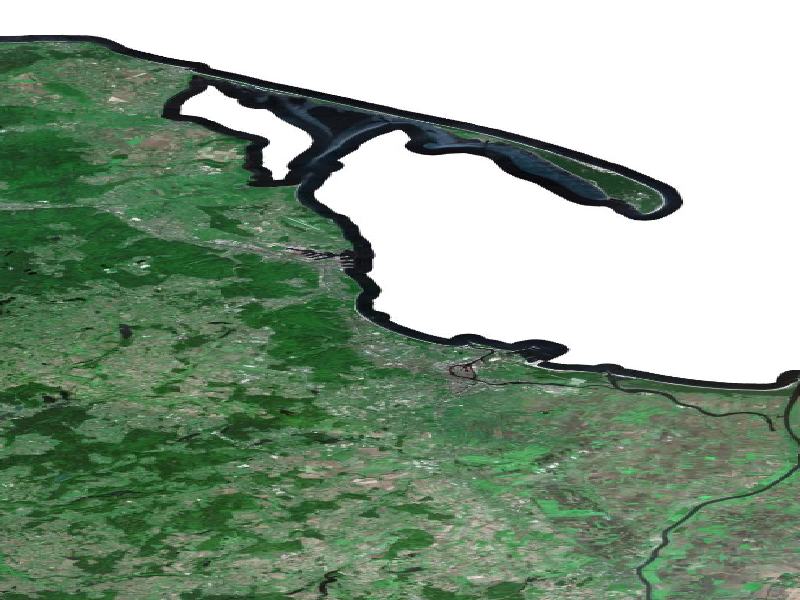
\includegraphics[width=0.7\textwidth]{img/pomorze_gdanskie.png}
    \caption{Pomorze Gdańskie zwrócone przez geoportal}
    \label{fig:pomorze_gdanskie}
\end{figure}

\subsection{WFS}

W ostatnich latach obserwuje się rosące zapotrzebowanie na usługi oparte na danych geograficznych takie jak nawigacja \cite{TRZEBA_COS_ZNALEZC}.
W celu realizacji takich usług, konieczne jest otrzymanie mapy w formacie innym niż rastrowy czy wektorowy, w celu jej dalszego przetworzenia.
Ponadto, w dobie urządzeń mobilnych, możliwość wprowadzania poprawek do danych z dowolnego miejsca wydaje się być koniecznością.
Odpowiedzią na te dwie potrzeby jest standrad Web Feature Service.
Opisuje on, w jaki sposób przesyłać i edytować dane zapisane w metajęzyku GML za pomocą protokołu HTTP.

Metajęzyk Geography Markup Language GML jest sposobem na zapis informacji geograficznych opartym na formacie XML (formalnie rzecz biorąc, jest gramatyką dla XMLa).
Jak każda gramatyka dla XMLa, definiuje plik schematu (XML schema). Są w nim określone następujące typy węzłów:
\begin{itemize}
    \item Feature
    \item Geometry
    \item Coordinate reference system
    \item Topology
    \item Time
    \item Dynamic feature
    \item Coverage (including geographic images)
    \item Unit of measure
    \item Directions
    \item Observations
    \item Map presentation styling rules
\end{itemize}

W ramach typu \textit{geometry}, zdefiniowano 3 rodzaje geometri: punkty, linie łamane oraz wielokaty.
Ponadto, społeczności skupione wokół tych samych projektów często definiują własne typy geometryczne, takie jak drogi.
Przykładowy fragment pliku GML:

\begin{lstlisting}[frame=L, language=xml]
<gml:Point>
    <gml:posList>
        50,100
    </gml:posList>
</gml:Point>
<gml:LineString>
    <gml:posList>
        50,100 100,150
    </gml:posList>
</gml:LineString>
<gml:Polygon>
    <gml:outerBoundaryls>
        <gml:LinearRing>
            <gml:posList>
                10,10 20,10 20,20 10,20 10,10
            </gml:posList>
        </gml:LinearRing>
    </gml:outerBoundaryls>
</gml:Polygon>
\end{lstlisting}

Co więcej, GML dopuszcza także korzystanie z profili. Pozwalają one na uproszczenie tworzenia plików GML. Aby z nich skorzystać, należy je zaimportować \cite{OpeGIS_GML2007}.
Istnieje także język KML, który jest propozycją uproszczenia GMLa. Jest wykorzystywany w usługach geograficznych firmy Google \cite{kulawiak2014}.

Jak wspomniano wyżej, sposób pobierania i edytowania plików GML opisuje standard WFS. Definiuje on zestaw rządań, na które musi odpowiedzieć serwer.
Rządania te mogą być przesyłane za pomocą przeglądarki internetowej. Ponadto, standard dopuszcza używanie zapytań (query). Pozwalają one
na filtrowanie danych dostępnych na serwerze, a następnie na takim podzbiorze danych wykonanie jednego ze zdefiniowanych zapytań \cite{OpenGIS_WFS2010}.
Lista rządań prezentuje się następująco:
\begin{itemize}
    \item GetCapabilities - zwraca informacje opisujące serwer (m.in. jego zawartość);
    \item DescribeFeatureType - zwraca informacje o schematach opisujące niestandarddowe typy (np: drogi) dostępnych na danym serwerze;
    \item GetPropertyValue - informację o wartości konkretnego pola we wszystkich obiektach uzyskanych za pomocą zapytania;
    \item GetFeature - zwraca obiekty na podstawie zapytania;
    \item LockFeature - pozwala na zablokowanie dostępu do zbioru obiektów. Działa podobnie do mechanizmu blokowania znanego z relacyjnych
        baz danych.
    \item GetFeatureWithLock - podobnie jak GetFeature, lecz poza zwróceniem obiektów powienien je również zablokować;
    \item Transaction - służy do tworzenie, zmieniania, zastępowania i usuwania obiektów z serwera;
    \item CreateStoredQuery - zapisuje nowe zapytanie na serwerze;
    \item DropStoredQuery - usuwa zapytanie z serwera;
    \item ListStoredQueries - wypisuje zapytania zapisane na serwerze;
    \item DescribeStoredQueries - zwraca metadane dotyczące wszystkich zapytań zapisanych na serwerze.
\end{itemize}

Przykładowe zapytanie i odpowiedź serwera:
\begin{lstlisting}[frame=L, language=XML]
<!-- Zapytanie -->
<?xml version="1.0" ?>
<GetFeature
    version="2.0.0"
    service="WFS"
    xmlns="http://www.opengis.net/wfs/2.0"
    xmlns:fes="http://www.opengis.net/fes/2.0"
    xmlns:myns="http://www.someserver.com/myns"
    xmlns:xsi="http://www.w3.org/2001/XMLSchema-instance"
    xsi:schemaLocation="http://schemas.opengis.net/wfs/2.0.0/wfs.xsd">
    <Query typeNames="myns:InWaterA_1M">
    <wfs:PropertyName>myns:wkbGeom</wfs:PropertyName>
    <wfs:PropertyName>myns:tileId</wfs:PropertyName>
    <fes:Filter>
        <fes:ResourceId rid="InWaterA_1M.1013"/>
        <fes:ResourceId rid="InWaterA_1M.1014"/>
        <fes:ResourceId rid="InWaterA_1M.1015"/>
    </fes:Filter>
    </Query>
</GetFeature>

<!-- Odpowiedź (fragment) -->

<wfs:member>
    <InWaterA_1M gml:id="InWaterA_1M.1014">
        <wkbGeom>
            <gml:Polygon srsName="urn:ogc:def:crs:EPSG::4326" gml:id="P2">
                <gml:exterior>
                    <gml:LinearRing>
                        <gml:posList>
                        -30.92013931274414 117.6552810668945 -30.92383384704589
                        117.661361694336 -30.93005561828613 117.6666412353516
                        -30.93280601501464 117.6663589477539 -30.93186187744141
                        117.6594467163086 -30.93780517578125 117.6541137695312
                        -30.94397163391114 117.6519470214844 -30.94255638122559
                        117.6455535888672 -30.93402862548828 117.6336364746094
                        -30.92874908447266 117.6355285644531 -30.92138862609864
                        117.6326370239258 -30.92236137390137 117.6395568847656
                        -30.91708374023438 117.6433029174805 -30.91711044311523
                        117.6454467773437 -30.92061042785645 117.6484985351563
                        -30.92061042785645 117.6504135131836 -30.91638946533203
                        117.6504440307617 -30.92013931274414 117.6552810668945
                        </gml:posList>
                    </gml:LinearRing>
                </gml:exterior>
            </gml:Polygon>
        </wkbGeom>
        <id>28021</id>
        <tileId>177</tileId>
    </InWaterA_1M>
</wfs:member> 
\end{lstlisting}

\subsection{WCS}

Dzięki usługom opartym o standrady WMS i WFS możliwe jest przeglądanie, przetwarzanie i edytowanie danych geograficznych.
Rozwój algorytmów służących do przetwarzania danych geograficznych (patrz rozdział 2), powoduje powstawanie dużej ilości danych w postaci pokryć macierzowych
(z ang. \textit{coverages}). Zwykle są to zdjęcia lotnicze i satelitarne, ale mogą też być to chmury punktów czy też numeryczne modele terenu \cite{sudra2012}.
Aby umożliwić dostęp do tego typu informacji, stworzono standrad Web Coverage Service WCS.

W porównaniu do WMS, który przedstawia dane w postaci statycznych map (obrazków), WCS zwraca dane razem z ich opisem oraz semantyką.
Pozwala to na analizowanie, ekstrapolowanie itp. danych, a nie tylko ich wyświetalnie.
W przeciweństwie do WFS, który zwraca dyskretne dane dotyczące zjawisk geograficznych, WFC przedstawia dane w sposób ciągły.
Serwery WCS mogą dostarczać dane w różnych formatach, w szczególności DTED, GeoTIFF, NTF, HDF-EOS i GML. Podobnie jak standard WMS,
WCS także definiuje 3 zapytania \cite{OpenGIS_WCS2012}:
\begin{itemize}
    \item GetCapabilities - zwraca informacje opisujące serwer (m.in. jego zawartość);
    \item DescribeCoverage - zwraca listę wszystkich dostępnych pokryć macierzowych wraz z ich opisami;
    \item GetCoverage - zwraca rządane pokrycie macierzowe.
\end{itemize}

\section{GeoServer i MapServer}

Istnieją różne technologie dostępu do danych geograficznych, jak chociażby opisane w \autoref{chap:protokoly} standardy WMS, WFS i WCS.
Jednakże są to tylko standardy. Konieczne jest stworzenie oprogramowania, które będzie je implementowało, a tym samym umożliwi
uzytkownikom dostęp do danych. GeoServer oraz MapServer są przykładami takiego oprogramowania.

GeoServer jest serwerem pozwalającym na pozyskiwanie i edytowanie danych geograficznych.
Jest napisany w języku Java jako oprogramowanie typu open-source.
Jako tego typu projekt, jest tworzony, testowany i rozwijany przez grupę osób i organizacji rozsianych po całym świecie.
GeoServer stanowi referencyjną implementację standardów WFS i WCS. Ponadto posiada certyfikat wysokiej wydajności implementacji WMSa.
Serwer ten obsługuje dane geograficzne różnych rodzajów, w tym formaty bazodanowe (PostGIS, Oracle Spatial) jak i plikowe (Shapefiles, GeoTIFF)
jako źródła danych. Poza tym możliwe jest też wykorzystanie innego serwera WMS czy WFS jako źródła.
Format danych zwracanych zależny jest od wykorzystywanego protokołu. Dodatkowo, wraz z serwerem dostarczana jest wbudawana aplikacja
oparta na OpenLayers (\ref{chap:OpenLayers}), która umożliwia podgląd umieszczanych map bez konieczności poznawania składni zapytań \cite{GeoServerManual2016}.

GeoServer nie istnieje w próżni. Do jego działania konieczna jest baza danych (w tym przypadku PostGIS). Dodatkowo istnieje też usługa
GeoWebCache, która zapisuje odpowiedzi na zapytania. Przyspiesza to działanie serwera z punktu widzenia użytkownika, który nie musi
czekać na wygenerowanie odpowiedzi \cite{OpenGeo2012}. Na rysunku \ref{fig:GeoServerArchitecture} przedstawiono tę architekturę, wraz z zaznaczoną
aplikacją użytkownika.

\begin{figure}[h!]
    \centering
    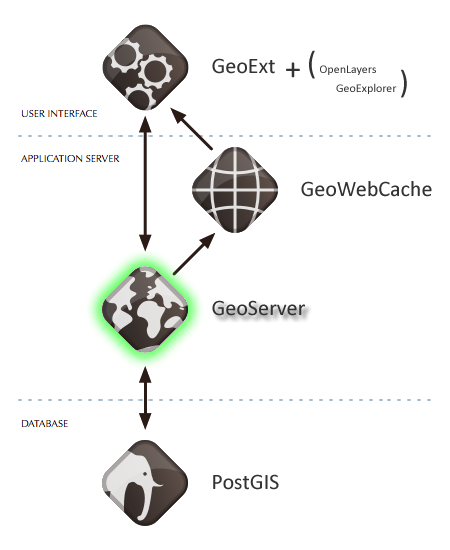
\includegraphics[width=0.4\textwidth]{img/geoserver_architecture.png}
    \caption{Architektura GeoServer}
    \source{http://presentations.opengeo.org/2012\_FOSSGIS/suiteintro/\_images/stack\_geoserver.png}
    \label{fig:GeoServerArchitecture}
\end{figure}

Jak wspomniano wyżej, GeoServer obsługuje wiele różnych standardów OGC, w tym WMS. W momencie przyjścia rządania o dostarczenie mapy,
serwer wykonuje następujące operacje:
\begin{enumerate}
    \item Ładowanie danych z bazy (opcjonalne filtrowanie)
    \item Nałożenie stylu
    \item Renderowanie obrazka i zwrócenie do użytkownika
\end{enumerate}
Na rysunku \ref{fig:geoserver_WMS_architecture} przedstawiono jak przebiega ten proces.

\begin{figure}[h!]
    \centering
    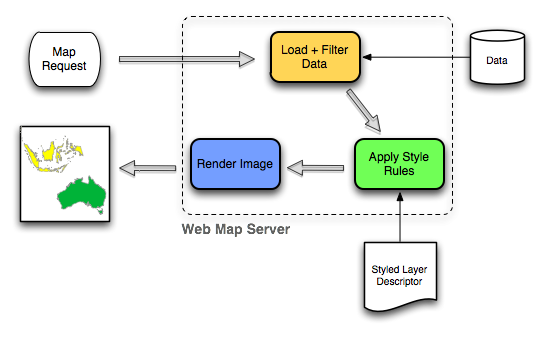
\includegraphics[width=0.7\textwidth]{img/geoserver_wms_architecture.png}
    \caption{Schemat odpowiedzi GeoServera na zapytanie GetMap}
    \source{http://presentations.opengeo.org/2012\_FOSSGIS/suiteintro/\_images/wms.png}
    \label{fig:geoserver_WMS_architecture}
\end{figure}

Obsługa GeoServera możliwa jest z poziomu przeglądarki. Nie ma konieczności edytowania plików konfiguracyjnych
w celu dodania nowego źródła danych, utworzenia nowej warstwy czy zdefiniowania nowego stylu. Dzięki temu rozwiązaniu
GeoServer może być łatwo wykorzystywany także przez użytkowników nie zaznajomionych z obsługą typowych aplikacji serwerowych.
Na rysunku \ref{} przedstawiono interfejs WWW dostarczany przez GeoServer.

MapServer stanowi alternatywę dla GeoServera. Podobnie jak poprzednik, MapServer stanowi implementację różnych standardów,
w tym WMS, WFS i WCS. Jest napisany w języku C/C++. Rozwijany jest przez wiele firm z całego świata jako projekt open-source.
Podstawowoym źródłem danych dla MapServera są pliki shapefile, ale możliwe jest też wykorzystanie innych źródeł. 
Moożliwe jest też wykorzystanie innego serwera WMS czy WFS jako źródła danych \cite{MapServer2011}.
Format danych zwracanych jest zależny od wybranego protokołu.

Najprostsza aplikacja oparta o MapServer składa się z następujących komponentów:
\begin{itemize}
    \item Dane wejściowe - mogące pochodzić z loklanych baz danych, jak i zewnętrznych serwerów;
    \item Aplikacje MapServer i MapScript - odpowiedzialne za obsługe rządania. Ich konfiguracja zawarta jest w plikach Mapfile
    \item Serwer WWW (Apache) - odpowiada za komunikację poprzez protokół HTTP z klientem
\end{itemize}

Architektura ta została przedstawiona na rysunku \ref{fig:mapserver_architecture}.
\begin{figure}[h!]
    \centering
    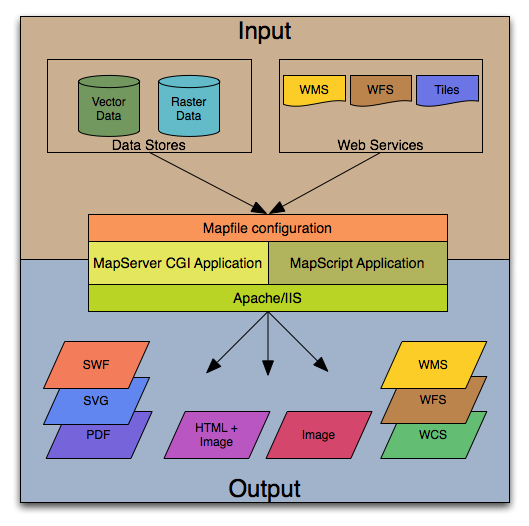
\includegraphics[width=0.7\textwidth]{img/mapserver_architecture.png}
    \caption{Architektura MapServera}
    \source{http://mapserver.org/\_images/architecture.png}
    \label{fig:mapserver_architecture}
\end{figure}

W przeciwieństwie do GeoServera, MapServer nie posiada interfejsu graficznego. Wszystkie operacje takie jak,
dodanie nowej mapy, zmiana stylu czy dodanie nowej warstwy, muszą być być przeprowadzane przy użyciu plików
konfiguracyjnych typu Mapfile (.map). Są to pliki tektowe, których konwencja przypomina tą znaną z plików
konfiguracyjnych dla serwisów działających w systemach linux. W ramach pliku mapfile można zdefiniować następujące
obiekty \cite{MapServer2011}:
\begin{itemize}
    \item MAP - obiekt odzwierciedlający całą mapę;
    \item LAYER - obiekt odzwierciedlający warstwę mapy. Musi być typu \textit{RASTER}, wtedy warstwa bedzie warstwą rastrową,
        bądź typu \textit{POINT, LINE} lub \textit{POLYGON} - wtedy warstwa będzie warstwą wektorową;
    \item CLASS - obiekt przechowujący dane dotyczące styli;
    \item SYMBOL - symbol do umieszczenia na mapie;
    \item LABEL - umożliwia dodanie napisu na mapie.
\end{itemize}

Poniżej przedstawiono przykładowy plik konfiguracyjny wraz ze zwróconą mapą (rysunek \ref{fig:mapserver_config}).

\begin{lstlisting}[frame=L]
MAP
    NAME "sample"
    STATUS ON
    SIZE 600 400
    SYMBOLSET "../etc/symbols.txt"
    EXTENT -180 -90 180 90
    UNITS DD
    SHAPEPATH "../data"
    IMAGECOLOR 255 255 255
    FONTSET "../etc/fonts.txt"

    #
    # Start of web interface definition
    #
    WEB
        IMAGEPATH "/ms4w/tmp/ms_tmp/"
        IMAGEURL "/ms_tmp/"
    END # WEB

    #
    # Start of layer definitions
    #
    LAYER
        NAME 'global-raster'
        TYPE RASTER
        STATUS DEFAULT
        DATA bluemarble.gif
    END # LAYER
END # MAP
\end{lstlisting}

\begin{figure}[h!]
    \centering
    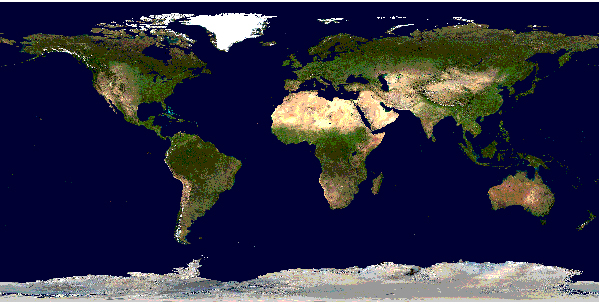
\includegraphics[width=0.7\textwidth]{img/mapserver_config.jpg}
    \caption{Przykładowa odpowiedź od MapServera}
    \source{http://mapserver.org/\_images/bluemarble-rendered.jpg}
    \label{fig:mapserver_config}
\end{figure}

\section{OpenLayers i Leaflet.js}
\label{chap:OpenLayers}

W poprzednim rozdziale opisano dwa konkurencyjne rozwiązania serwerowe, które, ogólnie rzecz ujmując, służą do dostarczania danych geograficznych użytkownikowi.
Do komunikacji z takim serwerem, konieczne jest posiadanie odpowiedniego klienta. Zgodnie ze standardami OCG \cite{OpenGIS_WMS2006,OpenGIS_WFS2010,OpenGIS_WCS2012}
komunikacja możliwa jest przy użyciu przeglądarki internetowej. Jednakże, ręczne tworzenie zapytań jest długotrwałe i mało wygodne. Dlatego powstały biblioteki
dla języka JavaScript, ułatwiające komunikację z serwerami WMS, WFS i WCS. W tym podrozdziale zostaną opisane dwie z nich - OpenLayers i Leaflet.js

OpenLayers powstało w 2006 roku jako odpowiedź na pojawienie się zamkniętych Google maps.
Za cel postawiono umożliwienie użytkownikom wyświetlania na swoich stronach map w sposób podobny do tego, znanego z usług Google.
Jednakże projekt miał umożliwiać tworzenie map z dowolnego źródła i miał być open-sourcowy \cite{website:OpenLayersHistory}.
Akutalnie rozwiajana jest wersja 3 biblioteki, pomimo że sporo aplikacji ciągle używa poprzedniej wersji.

Aplikacja wykorzystująca OpenLayers może korzystać ze źródeł w wielu formatach. Należą do nich:
\begin{itemize}
    \item Źródła dostarczające dane w formacie kafelkowym np: OSM, Bing;
    \item Dane wektorowe w formatach GeoJSON, TopoJSON, KML i GML;
    \item Dane dostarczane przez serwer zgodny ze standardami OGC.
\end{itemize}

Aplikacje korzystające z OpenLayers wykorzystują pewne standardowe komponenty dostarczane przez bibliotekę. Podstawowym jest mapa (\textit{ol.map}).
Jest ona rysowana w obiekcie celu (\textit{target}). Parametry obiektu mapy mogą być określane przy jej inicjalizacji lub po jej utworzeniu.
Obiekt mapy nie jest odpowiedzialny za oddalanie, przybliżanie czy przesuwanie mapy. Do tego celu służy obiekt widoku(\textit{ol.View}).
Dodatkwo należy zdefiniować źródło danych (\textit{ol.source.Source}). 
Aby wyświetlić dane ze źródła, potrzebny jest obiekt warstwy (\textit{ol.layer}). Aktualnie istnieją 3 rodzaje warstw:
\begin{itemize}
    \item \textit{ol.layer.Tile} - rodzaj warstwy dla danych w postaci gotowych kafelków;
    \item \textit{ol.layer.Image} - rodzaj warstwy do wyświetlania obrazków;
    \item \textit{ol.layer.Vector} - rodzaj warstwy do wyświetlania danych wektorowych.
\end{itemize}

Oczywiście, na jednej mapie może być dowolnie wiele warstw. Wykorzystując opisane komponenty można stworzyć taką przykładową aplikację:

\begin{lstlisting}[frame=L, language=JavaScript]
<div id="map" style="width: 100\%,height:400px"></div>
<script>
  new ol.Map({
    layers: [
      new ol.layer.Tile({source: new ol.source.OSM()})
    ],
    view: new ol.View({
      center: [0, 0],
      zoom: 2
    }),
    target: 'map'
  });
</script>
\end{lstlisting}

Wynik działania tej aplikacji przedstawiono na rysunku \ref{fig:openlayers_example}.

\begin{figure}[h!]
    \centering
    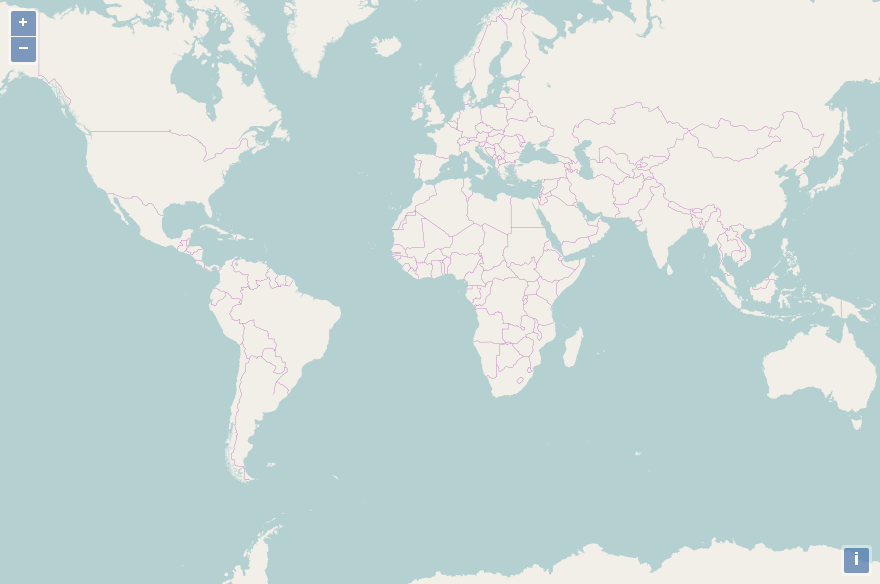
\includegraphics[width=1.0\textwidth]{img/openlayers_example.png}
    \caption{Przykładowa aplikacja OpenLayers}
    \source{własne}
    \label{fig:openlayers_example}
\end{figure}

